% Chapter 3

\chapter{Iterative Techniques for Mixed-Integer Linear Programming Problems} % Main chapter title

\label{Chapter3} % For referencing the chapter elsewhere, use \ref{Chapter2} 
%%%%%%%%%%%%%%%%%%%%%%%%%%%%%%%%%%%%%%%%%%%%%%%%%%%%%%%%%%%%%%%%%%%%%%%%%%%%%%%

%%%%%%%%%%%%%%%%%%%%%%%%%%%%%%%%%%%%%%%%%%%%%%%%%%%%%%%%%%%%%%%%%%%%%%%%%%%%%%%
As we stated in previous chapters, quantum computers are not mature enough to solve real-world problems. For instance, the embedding of a QUBO problem into the architecture of a quantum annealer imposes a big constraint in the number of variables our problem can have. For this reason, a \textit{hybrid quantum-classical} (HQC) approach is currently the best method one can use to tackle large-scale problems, by combining quantum and classical solvers.\\\\
The aim of HQC approaches is to decompose a problem into a \textit{sub-problem(s)} (SP(s)) and a \textit{master problem} (MP), with the hope that one of these problems is suitable for a quantum computer. On the one hand, a quantum annealer receives a QUBO problem or a problem that can be cast into it. On the other, the other problems are solved by the classical solver using cutting-edge algorithms. The MP and SP(s) are solved iteratively until a given stopping criterion is satisfied. \\\\
There are classical systematic approaches that always converge for convex functions, such as the Benders' decomposition algorithm\,\cite{Pereira1991}, while other heuristic approaches do not guarantee the optimal solution, but they require less computational resources to find a sub-optimal solution by exploring the configuration space according to some criteria.\\\\
In this chapter, we describe the general formulation of a mixed-integer linear programming problem, then we present the most relevant results of dual dynamic programming theory which is the underlying theory of problem decomposition. Finally we show a quantum-classical Benders' decomposition protocol\,\cite{Zhao2021HybridProgramming}, a heuristic quantum-classical protocol\,\cite{Ding2019ImplementationDesign} and another version inspired on it.
%%%%%%%%%%%%%%%%%%%%%%%%%%%%%%%%%%%%%%%%%%%%%%%%%%%%%%%%%%%%%%
% MILP
%%%%%%%%%%%%%%%%%%%%%%%%%%%%%%%%%%%%%%%%%%%%%%%%%%%%%%%%%%%%%%
\newpage
\section{Mixed-Integer Linear Programming}
In the present work, we are interested in mixed-integer linear programming (MILP) problems because they appear in a wide range of real-world applications and they are the corresponding mathematical formulation of TEP problems. More precisely, TEP problems contain real variables but these variables are often converted into integer values to solve the problem.\\\\
The general mathematical formulation of MILP problems is
\begin{mini!}[2]
	{\mathbf{x}}{f(\mathbf{x})}{\label{eq: MILP}}{}{\left[f: \mathbb{R}^{n} \rightarrow \mathbb{R}\right]}
	\addConstraint{h(\mathbf{x})}{=0,}{\left[h: \mathbb{R}^{n} \rightarrow \mathbb{R}^{m}\right]}
	\addConstraint{g(\mathbf{x})}{\leq 0,\quad}{\left[g: \mathbb{R}^{n} \rightarrow \mathbb{R}^{p}\right],}
\end{mini!}
where $m$ and $p$ are the number of equality and inequality constraints and $\mathbf{x}$ are the decision variables.\\\\
TEP problems scale badly as the problem size grows. Thus, big problems cannot be solved at the desired resolution by nowadays classical computers with solvers such as Gurobi\,\cite{gurobi}, CPLEX\,\cite{cplex2009v12} or cbc\,\cite{cbc}. There are already benchmarks comparing classical solvers and quantum annealers for energy problems where even the fastest of these solvers -- Gurobi -- cannot find the optimal solution in a fixed run-time, see Ref.\,\cite{Fernandez-Campoamor2021CommunityAnnealing}. \\\\
%%%%%%%%%%%%%%%%%%%%%%%%%%%%%%%%%%%%%%%%%%%%%%%%%%%%%%%%%%%%%%%%%%
% Classical Benders Decomposition
%%%%%%%%%%%%%
\section{Classical Benders' Decomposition}
The main idea behind classical \textit{Benders' decomposition} (BD) -- also known as \textit{dual dynamic programming} (DDP) -- is to decompose the primal problem into a master problem and a sub-problem(s) once the complicated variables are detected. In the following sections, we introduce the most relevant results of dual dynamic programming. For a deeper understanding see Ref.\,\cite{bierlaire2018}.
%%%%%%%%%%%%%
\subsection{Complicated Variables}
We can consider a decision variable to be complicated if the decision variable is involved in most of the constraints or the decision variable produces non-convex optimization problems. 
\begin{definition}{Complicated variables}
Those variables that allow us to split the original problem into sub-problem(s) when they are fixed. These variables appear in constraints in such a way that the problem cannot be decomposed if they are not fixed. These type of constraints are known as linking constraints. 
\end{definition}
After splitting the original problem, the master problem is a relaxed version of the original problem. The global minimum is guaranteed if and only if the objective function as a function of the complicated variables is a convex envelope.\\\\
For this reason, we propose BD to decompose the general problem \eqref{eq: MILP} into an MP with integer variables and an SP so that a clever rearrangement of the variables allows us to fix the complicated variables of the MP -- once the MP is solved -- and send these complicated variables as fixed for the sub-problem. This process is performed iteratively until a stopping criterion is satisfied. The convergence of BD\,\cite{Sahinidis1991BDConvergence} guarantees that we can satisfy an arbitrary threshold value after a number of iterations. 
%%%%%%%%%%%%%%%%%%%%%%%%%%%%%%
\subsection{Dual Dynamic Programming}
We can relax the primal problem by associating a penalty to each of its constraints,
\begin{equation}
    \lambda\in\mathbb{R}^{m}\,\, \text{and} \quad \mu\in\mathbb{R}^{p},
\end{equation}
also known as Lagrange multipliers. Then the Lagrangian of the primal problem is
\begin{equation}
    \mathcal{L}(\mathbf{x}, \lambda, \mu) = f(\mathbf{x}) + \lambda^{\intercal}h(\mathbf{x}) + \mu^{\intercal}g(\mathbf{x}).
\end{equation}
\begin{definition}{Dual function}{}
The dual function, $q: \left[\mathbb{R}^{m+p}\rightarrow\mathbb{R}\right]$, maps the set of parameters $\lambda$ and $\mu$ to a minimization problem
\begin{equation}
    q(\lambda, \mu) = \min_{\mathbf{x}\in\mathbb{R}^{n}}\mathcal{L}(\mathbf{x}, \lambda, \mu),
\end{equation}
where $m$ and $p$ are the number of equality and inequality constraints and
\begin{equation}
    \lambda\in\mathbb{R}^{m}\,\, \text{and} \quad \mu\in\mathbb{R}^{p},
\end{equation}
are the penalty parameters.
\end{definition}
Notice that the dual function is an unconstrained problem because all the constraints have been moved into the Lagrangian.
Considering the MILP problem \eqref{eq: MILP}, the inequality constraint $g(\mathbf{x})\leq 0$ is violated if $g(\mathbf{x})>0$. To take into account this in the cost function we need to introduce a positive cost, so $\mu^{\intercal}g(\mathbf{x})>0$ which implies $\mu^{\intercal}$ has positive coefficients, that is
\begin{equation}
    \mu \geq 0.
\end{equation}
\begin{theorem}{}{}
The dual of a linear optimization problem is another linear optimization problem.
\end{theorem}
\begin{theorem}{}{}
The dual of the dual is the primal.
\end{theorem}
\begin{theorem}{}{}
Suppose that $\mathbf{x}^{*}$ is an optimal solution -- so it is feasible -- of the primal. Then,
\begin{equation}
    q(\lambda, \mu) \leq f(\mathbf{x}^{*})
\end{equation}
is a lower bound of the primal problem, for
\begin{equation}
    \lambda\in\mathbb{R}^{m}\,\, \text{and} \quad \mu\in\mathbb{R}^{p}.
\end{equation}
\end{theorem}
\begin{proof}
\begin{align}
    q(\lambda, \mu) = \min_{\mathbf{x}\in \mathbb{R}^{n}} \mathcal{L}(\mathbf{x}, \lambda, \mu) \leq \mathcal{L}(\mathbf{x}^{*}, \lambda, \mu) = f(\mathbf{x}^{*}) + \underbrace{\lambda^{\intercal}h(\mathbf{x}^{*})}_{0} + \underbrace{\mu^{\intercal}g(\mathbf{x}^{*})}_{\leq 0} \leq f(\mathbf{x}^{*})
\end{align}
\end{proof}
A feasible solution satisfies the constraints, meaning that $h(\mathbf{x}^{*})=0$ and $g(\mathbf{x}^{*}) \leq 0$. This implies that the dual function $q(\lambda,\mu)$ is a lower bound and the relaxed problem $f(\mathbf{x}^{*})$ is the upper bound. Notice that if $\mu = 0$ then the lower bound and upper bound would have the same value. In DDP we need to optimize not only the decision variables $\mathbf{x}$ but also the penalty parameters $\mu$ and $\lambda$.
\begin{corollary}{}{}
  In particular, if $\mathbf{x}^{*}$ is an optimal solution of the primal and $\mathbf{x}$ is a feasible solution of the primal, then
  \begin{equation}
      \underbrace{q({\lambda,\mu})}_{\text{Lower Bound}} \leq f(\mathbf{x}^{*}) \leq \underbrace{f(\mathbf{x})}_{\text{Upper Bound}}
  \end{equation}
\end{corollary}
We want to find the best possible lower bound by solving the following optimization problem
\begin{maxi!}[2]
	{\lambda, \mu}{q(\lambda, \mu)}{\label{eq: Abstract_Dual}}{}{\left[q: \mathbb{R}^{m+p} \rightarrow \mathbb{R}\right]}
	\addConstraint{\mu}{\geq 0}{}
	\addConstraint{(\lambda, \mu)}{}{\in \{\lambda, \mu \,\mid\, q(\lambda, \mu) > - \infty \}.}
\end{maxi!}
Notice that we are choosing the penalties in such a way that the dual problem is bounded.
\begin{theorem}{Weak Duality}{}
If $\mathbf{x}^{*}$ is the optimal solution of the primal, and $\lambda^{*}, \mu^{*}$ is the optimal solution of the dual, then
\begin{equation}
    q(\lambda^{*}, \mu^{*}) \leq f(\mathbf{x}^{*})
\end{equation}
\end{theorem}
\begin{theorem}{Strong Duality}{}
If $\mathbf{x}^{*}$ is the optimal solution of the primal, and $\lambda^{*}, \mu^{*}$ is the optimal solution of the dual, then
\begin{equation}
    q(\lambda^{*}, \mu^{*}) = f(\mathbf{x}^{*})
\end{equation}
\end{theorem}
In other words, the strong duality theorem guarantees that the upper bound and lower bound are going to converge into a point for the optimal solution, see Figure\,\ref{fig:BD_Convergence}.
\begin{figure}[H]
\centering
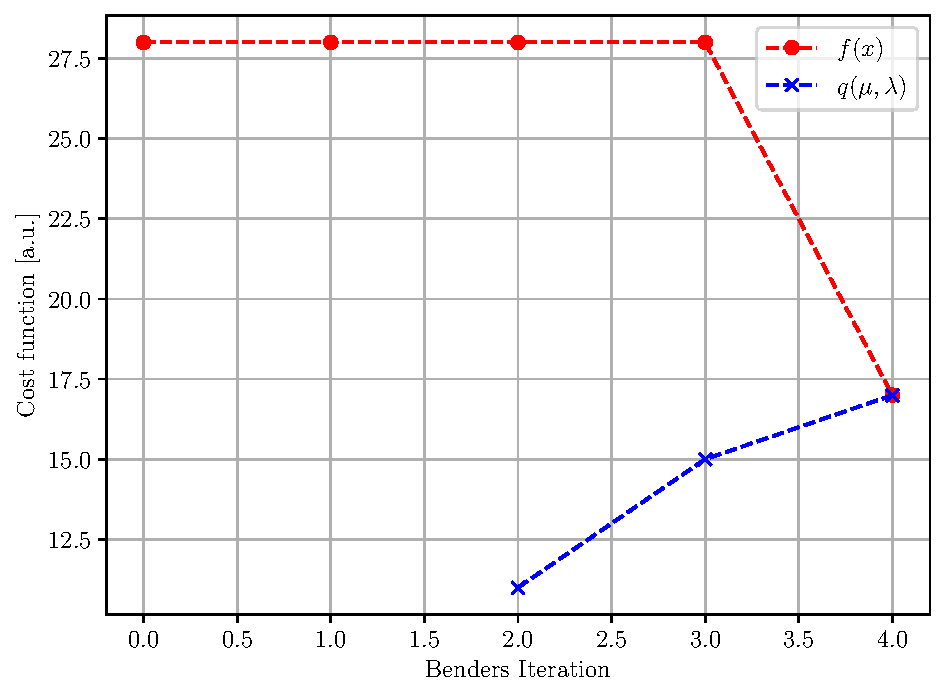
\includegraphics[width=0.8\textwidth]{Figures/BD_Convergence.pdf} 
\caption{Benders' decomposition convergence for a combinatorial problem in which the strong duality theorem is satisfied\,\cite{Zhao2021HybridProgramming}. Round indicates the number of iteration in the BD process and $t$ indicates}
\label{fig:BD_Convergence}
\end{figure}
\begin{corollary}{}{}
If either the primal problem or the dual problem are unbounded, then both problems are unbounded.
\end{corollary}
\begin{proof}
If the primal is unbounded, then according to the weak duality theorem
\begin{equation}
    q(\lambda^{*}, \mu^{*}) \leq \infty
\end{equation}
which implies the dual problem is unbounded. Analogously, if the dual problem is unbounded, then the primal problem is unbounded too.
\end{proof}
\begin{corollary}{}{}
If there exist $\mathbf{x}^{*},\lambda^{*}\,\text{and}\, \mu^{*}$ such that,
\begin{equation}
    q(\lambda^{*}, \mu^{*}) = f(\mathbf{x}^{*})
\end{equation}
then they are optimal.
\end{corollary}
\begin{proof}
Consider a feasible solution of the primal problem, $\mathbf{x}$, and a feasible solution of the dual problem, $(\lambda, \mu)$, then
\begin{equation}
    f(\mathbf{x}) \geq q(\lambda^{*}, \mu^{*}) = f(\mathbf{x}^{*}) \geq q(\lambda, \mu)
\end{equation}
\end{proof}
%%%%%%%%%%%%%%
\begin{figure}[H]
\centering
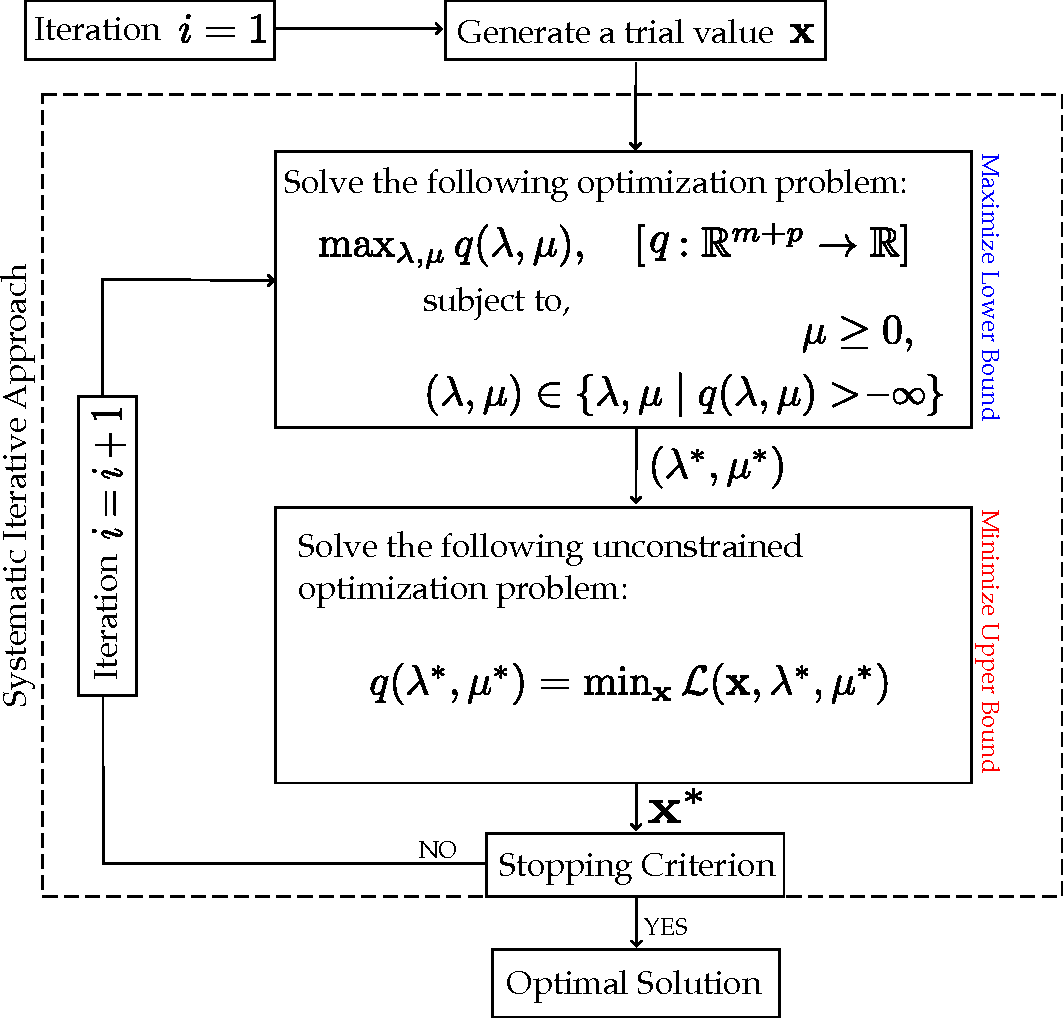
\includegraphics[width=\textwidth]{Figures/BDScheme.pdf} 
\caption{Benders' decomposition scheme. An iterative process is followed where the lower and upper bound are maximized and minimized, respectively, until a stopping criterion is satisfied.}
\label{fig:BDScheme}
\end{figure}
We conclude this section by summarizing Benders' decomposition algorithm. We propose a trial solution $\mathbf{x}$ that we feed into the dual problem and we maximize it, i.e., we find the $\lambda^{*}$ and $\mu^{*}$ that maximize the problem. The value of this problem generates a lower bound. Then we insert those optimal parameters $\lambda^{*}$ and $\mu^{*}$ in the Lagrange function and minimize it by finding $\mathbf{x}^{*}$. Finally, if a given stopping criterion is satisfied, then we stop the iterative process, otherwise we update the dual problem with the new candidate solution $\mathbf{x}^{*}$ and repeat the algorithm. Figure \ref{fig:BDScheme} represents the iterative approach of BD.
%%%%%%%%%%%%%%%%%%%
\subsection{Benders' Decomposition: An Illustrative Example}
As an example, consider the general convex function of \ref{fig:BDIlustration},
\begin{equation}
    C(x_{3}) \propto x_{3}^{2}
\end{equation}
In each iteration of the BD scheme we are maximizing the lower bound -- dual problem -- and minimizing the upper bound -- primal problem --, graphically
\begin{figure}[H]
\centering
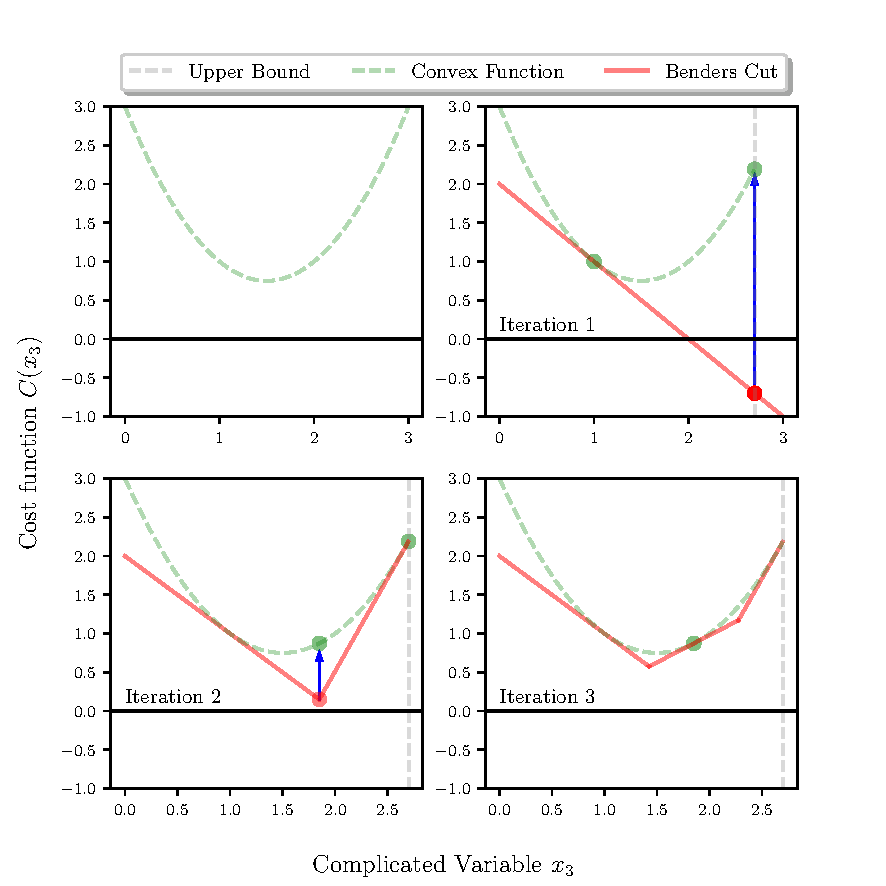
\includegraphics[width=\textwidth]{Figures/BenderIlustration.pdf} 
\caption{Graphical representation of BD protocol for a single complicated variable in an arbitrary convex function.}
\label{fig:BDIlustration}
\end{figure}
Benders' cuts are generated by updating the parameters $(\lambda,\mu)$ of the dual function. In other words, the iterative process restricts the feasible region until we get the optimal value.
%%%%%%%%%%%%%%%%%%%%%%%%%%%%%%%%%%%%%%%%%%%%%%%%%%%%%%%%%%%%%%%%%%%%%%%%%%%%%%%
% QA + SA
%%%%%%%%%%%%%%%%%%%%%%%%%%%%%%%%%%%%%%%%%%%%%%%%%%%%%%%%%%%%%%%%%%%%%%%%%%%%%%%
\section{Hybrid quantum-classical algorithms}
In Appx.\,\ref{AppendixB}, we show the foundations of \textit{simulated annealing} (SA) and solve a travelling salesman problem to illustrate it. A simulated annealing algorithm does not guarantee an optimal solution but the results we can get with a clever annealing schedule can be good enough in accuracy and time. The same applies to a quantum annealing algorithm. In this section, we show how the decomposition of a QUBO problem allows us to use both quantum and classical solvers, where the classical solvers relax the original problem so that it can be tackled by the quantum solver.
%%%%%%%%%%%%%%%%%%%%%%%%%%%%%%%%%%%%%%%%%%%%%%%%%%%%%%%%%%%%%%%%%%%%%%%%%%%%%%%
\subsection{Quantum Benders' Decomposition: Single Cuts}
The main idea behind the quantum Benders approach is to use the quantum annealer to solve either the primal problem or the dual problem. We are interested in solving the primal problem, also known as master problem, with a quantum annealer. The scheme is represented in Figure\,\ref{fig:BDScheme}. In our case, the candidate solution, $\mathbf{x}$, are generated by solving the minimization MP by a quantum annealer.
%%%%%%%%%%%%%%%%%%%%%%%%%%
\subsection{Heuristic Protocols}
As stated before, heuristic approaches do not guarantee to arrive at the optimal solution. However, these methods explore the configuration space in such a way that we do not get stuck in a local minimum. For a limited amount of computational resources and time, the solution that a heuristic approach can achieve is sub-optimal. Generally, these methods are better than a brute-force method when the problem is large enough so that there are no computational resources that are able to solve it by getting the optimal solution.
\subsubsection{SA-QA Protocol}
We present a hybrid quantum-classical algorithm protocol based on combining SA and QA\,\cite{Ding2019ImplementationDesign} to solve the MP and SP(s), respectively. Figure\,\ref{fig:SA_QAProtocol} shows a graphical representation of the SA-QA protocol, which we describe in more detail below. 
\begin{figure}[H]
\centering
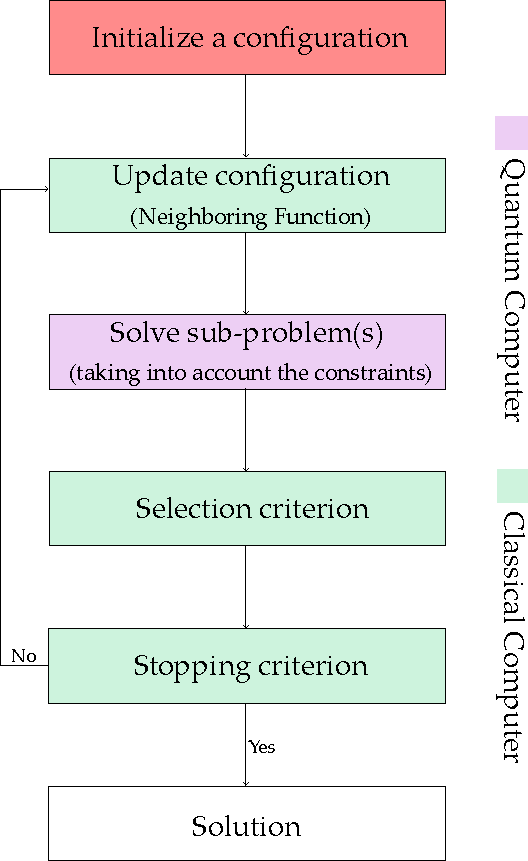
\includegraphics[width=0.45\textwidth]{Figures/SAQAProtocol_Layer 1.pdf} 
\caption{SA-QA scheme. See main text for details on this protocol.}
\label{fig:SA_QAProtocol}
\end{figure}
\begin{enumerate}
    \item Set the upper and lower bound of the problem -- so that we avoid dealing with unbound problems -- and initialize a configuration for the problem, i.e., annealing schedule, initial and final temperature, and a selection criterion.
    \item Randomly generate a new configuration by changing the values of the binary variables according to a neighboring function that generates a new configuration in one of these ways:
    \begin{enumerate}
        \item Randomly pick a binary variable with value 1 and set it to 0.
        \item Randomly pick a binary variable with value 0 and set it to 1.
        \item Randomly pick two binary variables with different values and swap them.
    \end{enumerate}
    \item Given the new configuration, solve the sub-problem(s) -- dual problems -- with a quantum annealing algorithm.
    \item Apply the selection criterion to keep or discard the current configuration.
    \item If the selection criterion is not satisfied, repeat steps 2 to 4 until a iteration index is equal to the value set in step 1, then decrease the temperature and reset the iteration index. If the selection criterion is satisfied, the protocol outputs the current cost function value and its solution $\mathbf{x}$.
\end{enumerate}
Notice that the algorithm solves the master problem with a simulating annealing algorithm in a classical solver and then the sub-problem(s) -- dual problems -- with the quantum computer, more precisely with a quantum annealer. For this reason, the sub-problem(s) must have binary constraints or low integer values if we do not want to deal with discretization errors or adding a big set of slack variables.\\\\
In order to apply both simulated and quantum annealing to problems in which the master problem contains most of the binary and integer variables -- as is the case with the TEP problem --, we have to reconsider or adapt the previous scheme.
%%%%%%%%%%%%%%%%%%%%%%%%%%%%%%%%%%%%%%%%%%%%%%%%%%%%%%%%%%%%%%
% QA-SA Protocol
%%%%%%%%%%%%%%%%%%%%%%%%%%%%%%%%%%%%%%%%%%%%%%%%%%%%%%%%%%%%%%
\subsubsection{QA-SA Protocol}
 As stated before, our sub-problem(s) has real constraints which implies it is not a clever approach to solve them with a quantum annealer. For this reason, we reverse the original protocol so that the quantum annealer tackles the master problem in which the binary and integer decision variables appear and the classical solver tackles the sub-problem(s). A scheme of the new protocol is shown in Figure\,\ref{fig:QA_SAProtocol}.\\\\
In order to explain the protocol in accordance to what has been shown in previous section we use the same notation $f(\mathbf{x})$ to describe the upper bound of the primal problem and $q(\lambda,\mu)$ to describe the lower bound, where $(\lambda,\mu)$ represents the penalties of our problem, in other words, the Lagrange multipliers, and $\mathbf{x}$ represent the decision variables. We are showing a heuristic approach, meaning that the convergence is not guaranteed. That is, we are not getting the optimal values $(\mathbf{x}^{*}, \lambda^{*},\mu^{*})$ that maximize the lower bound and minimize the upped bound in each iteration. Instead, we are optimizing the dual problem by SA algorithm and the master problem by QA, so that none of these methods guarantees the optimal solution to its combinatorial optimization problem.
\begin{figure}[H]
\centering
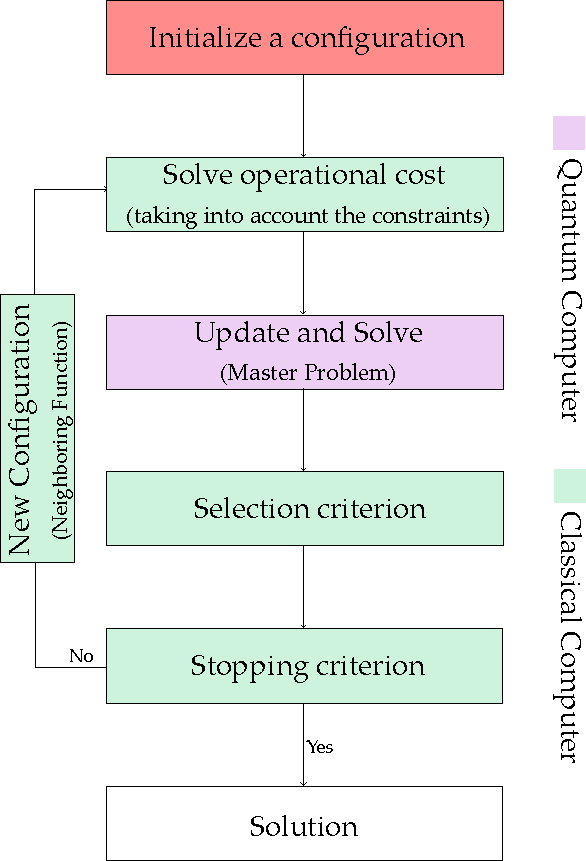
\includegraphics[width=0.5\textwidth]{Figures/QASAProtocol_Layer 1.pdf} 
\caption{QA-SA protocol scheme.}
\label{fig:QA_SAProtocol}
\end{figure}
\begin{enumerate}
    \item Set an initial feasible configuration to the primal problem $\mathbf{x}$.
    \item Solve the dual problem by SA,
\begin{maxi!}[2]
	{\lambda, \mu}{q(\lambda, \mu)}{}{}{\left[q: \mathbb{R}^{m+p} \rightarrow \mathbb{R}\right]}
	\addConstraint{\mu}{\geq 0}{}
	\addConstraint{(\lambda, \mu)}{}{\in \{\lambda, \mu \,/\mid, q(\lambda, \mu) > - \infty \}}.
\end{maxi!}
Notice that the parameters $\lambda$ and $\mu$ do not have to be the optimal parameters. SA does not guarantee to obtain the optimal solution of the dual problem.
    \item Update the master problem with $\{\lambda, \mu\}$ 
    \begin{equation}
        q(\lambda,\mu) = \min_{\mathbf{x}} \mathcal{L}(\mathbf{x}, \lambda, \mu).
    \end{equation}
     QA does not guarantee to obtain the optimal solution $\mathbf{x}^{*}$ of the master problem.
    \item Apply the selection criterion to keep or to discard the current configuration.
    \item If the stopping criterion is satisfied, then the protocol outputs the solution. Otherwise, insert the values $\mathbf{x}$ of step 3 into step 2 and repeat until step 4.
\end{enumerate}



